\setchapterstyle{lines}
\chapter[Not Simple Systems Equations]{Not Simple Systems Equations}
\labch{notSimpleSystems}

\renewcommand{\row}[2]{
	\multicolumn{2}{l}{#1} \\[+1mm]
	\small $#2$ & 
}
\renewcommand{\separation}{
			\multicolumn{2}{c}{}\\[-1em]
	        \hline
	        \multicolumn{2}{c}{}\\[-1em]
}

\begin{table}[!h] 
	\labtab{transferFunctions1}
	 	\begin{tabular}{>{\centering\arraybackslash}m{4cm} | >{\centering\arraybackslash}m{6.5cm}}
		        \hline
		        \multicolumn{2}{c}{}\\[-1em]
		        \row{Gear train, rotational transformer}{\dfrac{\omega_2}{\omega_1}=\dfrac{N_1}{N_2}} 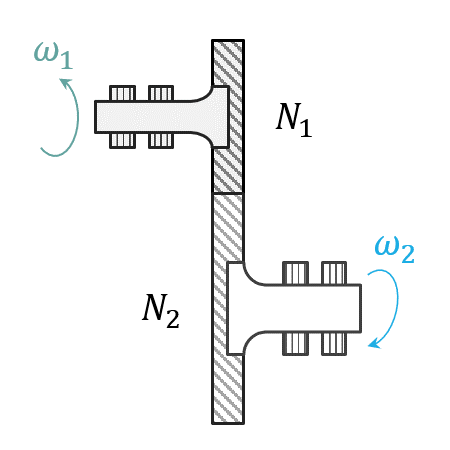
\includegraphics[height = 2.700 cm]{appendix_notSimpleSystemsEquations/Gear train} \\
		        \separation
				\row{Solenoid, magnetic force}{\dfrac{f_c}{i_c}=K_c} 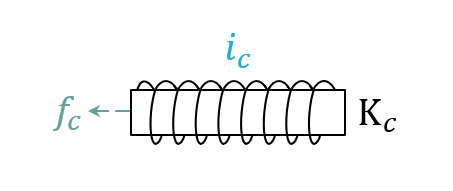
\includegraphics[height = 1.146 cm]{appendix_notSimpleSystemsEquations/Solenoid} \\
		        \separation
		        \row{Tachometer, velocity sensor}{\dfrac{v_t}{\omega_t}=K_t}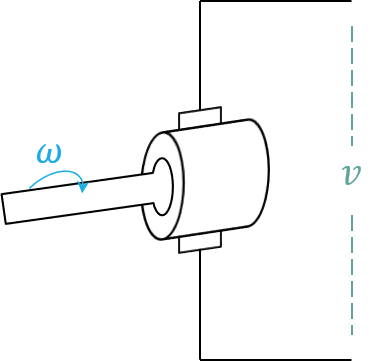
\includegraphics[height = 2.250 cm]{appendix_notSimpleSystemsEquations/Tachometer} \\
		        \separation
		        \row{AC motor, two-phase control field}{\dfrac{\Theta_m}{V_c}=\dfrac{K_m}{s(\tau_ms+1)}} 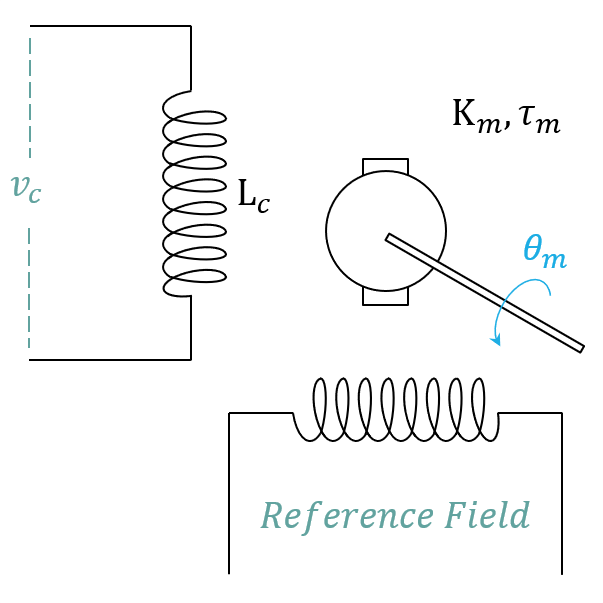
\includegraphics[height = 3.618 cm]{appendix_notSimpleSystemsEquations/AC motor} \\
		        \separation
		        \row{Amplidyne, rotary amplifier}{\dfrac{V_o}{V_c}=\dfrac{K_q}{sL_c+R_c}\cdot\dfrac{K_d}{sL_q+R_q}} 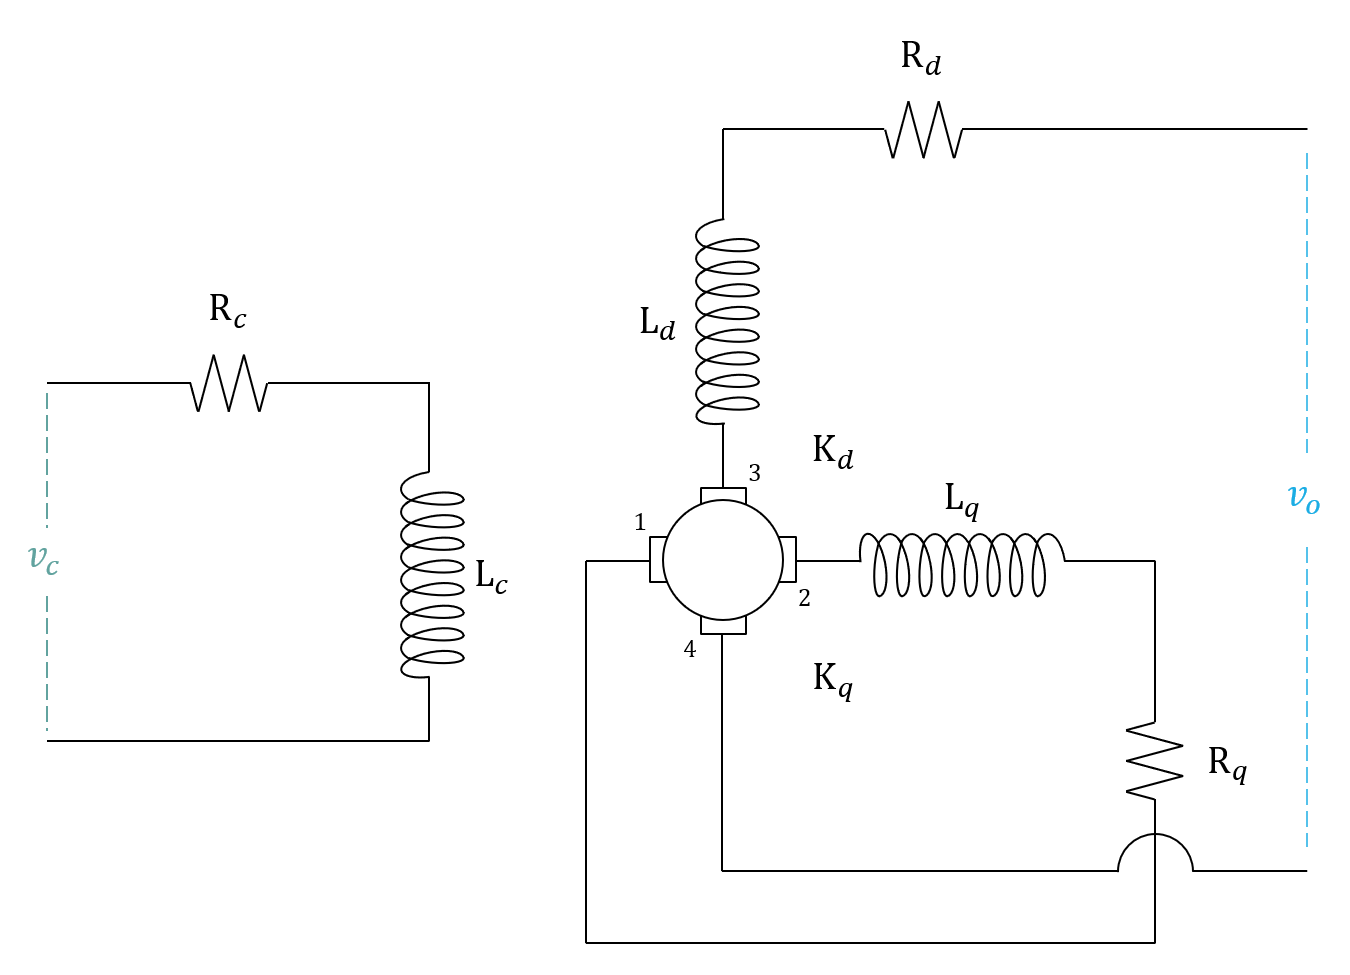
\includegraphics[height = 5.850 cm]{appendix_notSimpleSystemsEquations/Amplidyne} \\
		        \multicolumn{2}{c}{}\\[-1em]
		        \hline
		    \end{tabular}
\end{table}
\pagebreak


\begin{table}[!t]
	\caption{Transfer functions}
	\labtab{transferFunctions2}
	 	\begin{tabular}{>{\centering\arraybackslash}m{4cm} | >{\centering\arraybackslash}m{6.5cm}}
		        \hline
		        \multicolumn{2}{c}{}\\[-1em]
		        \row{DC amplifier, 0 Hz amplifier}{\dfrac{v_o}{v_i}=K_a} 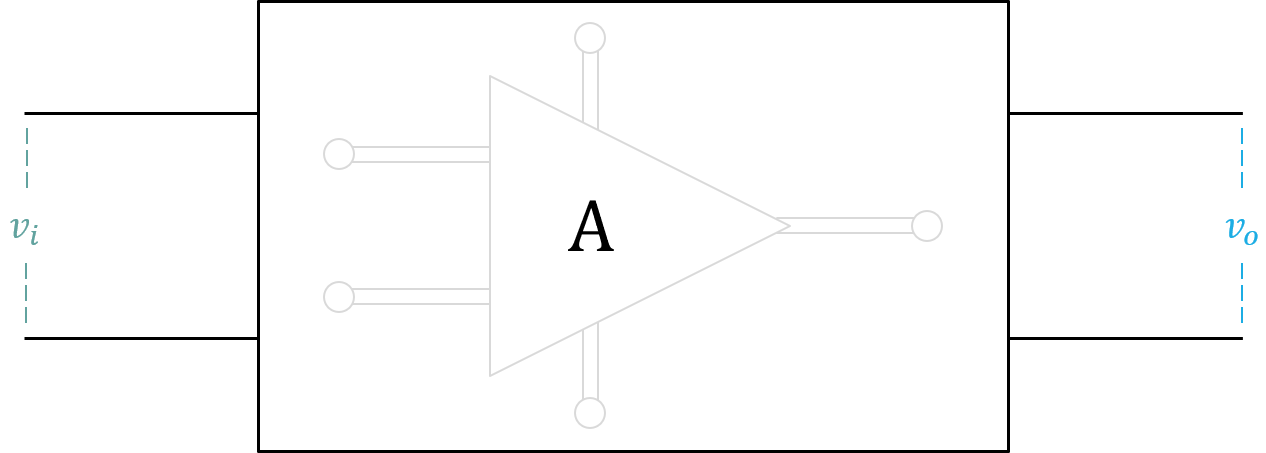
\includegraphics[height = 2.118 cm]{appendix_notSimpleSystemsEquations/DC amplifier} \\
		        \separation
		        \row{Demodulator, AC modulated signal to DC}{\dfrac{v_o}{v_i}=K_d} 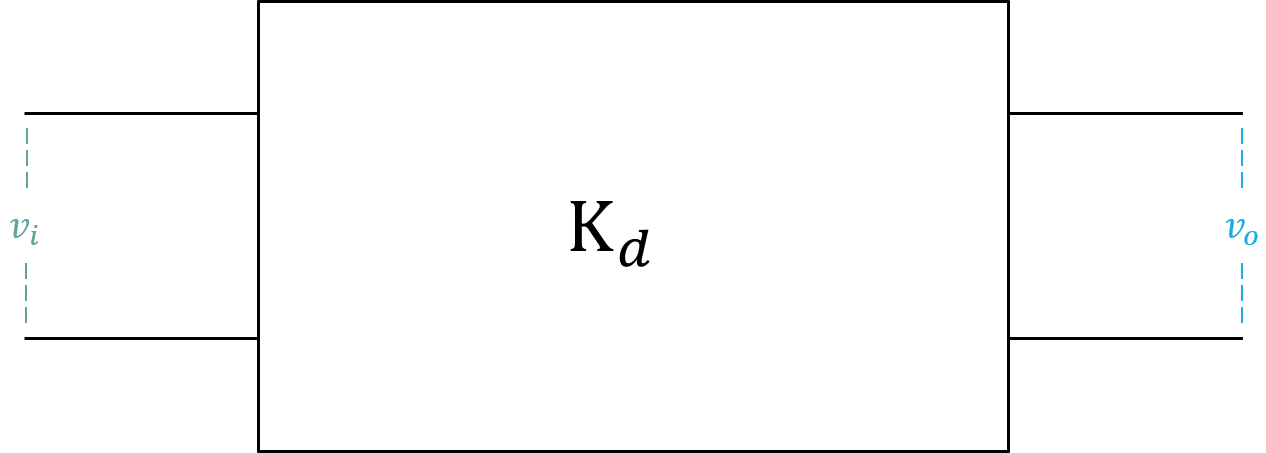
\includegraphics[height = 2.118 cm]{appendix_notSimpleSystemsEquations/Demodulator} \\
		        \separation
		        \row{Potentiometer, used in ``Error detector bridge''}{\dfrac{v_{error}}{\theta_r-\theta_c}=K_s} 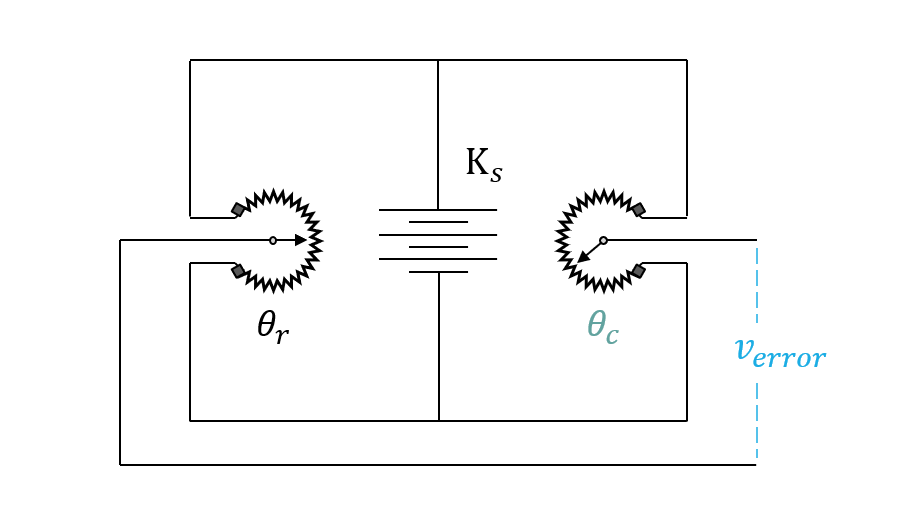
\includegraphics[height = 3.150 cm]{appendix_notSimpleSystemsEquations/Potentiometer} \\
		        \separation
		        \row{Synchro, as ``Error detector''}{\dfrac{v_{error}}{\theta_r-\theta_c}=K_s} 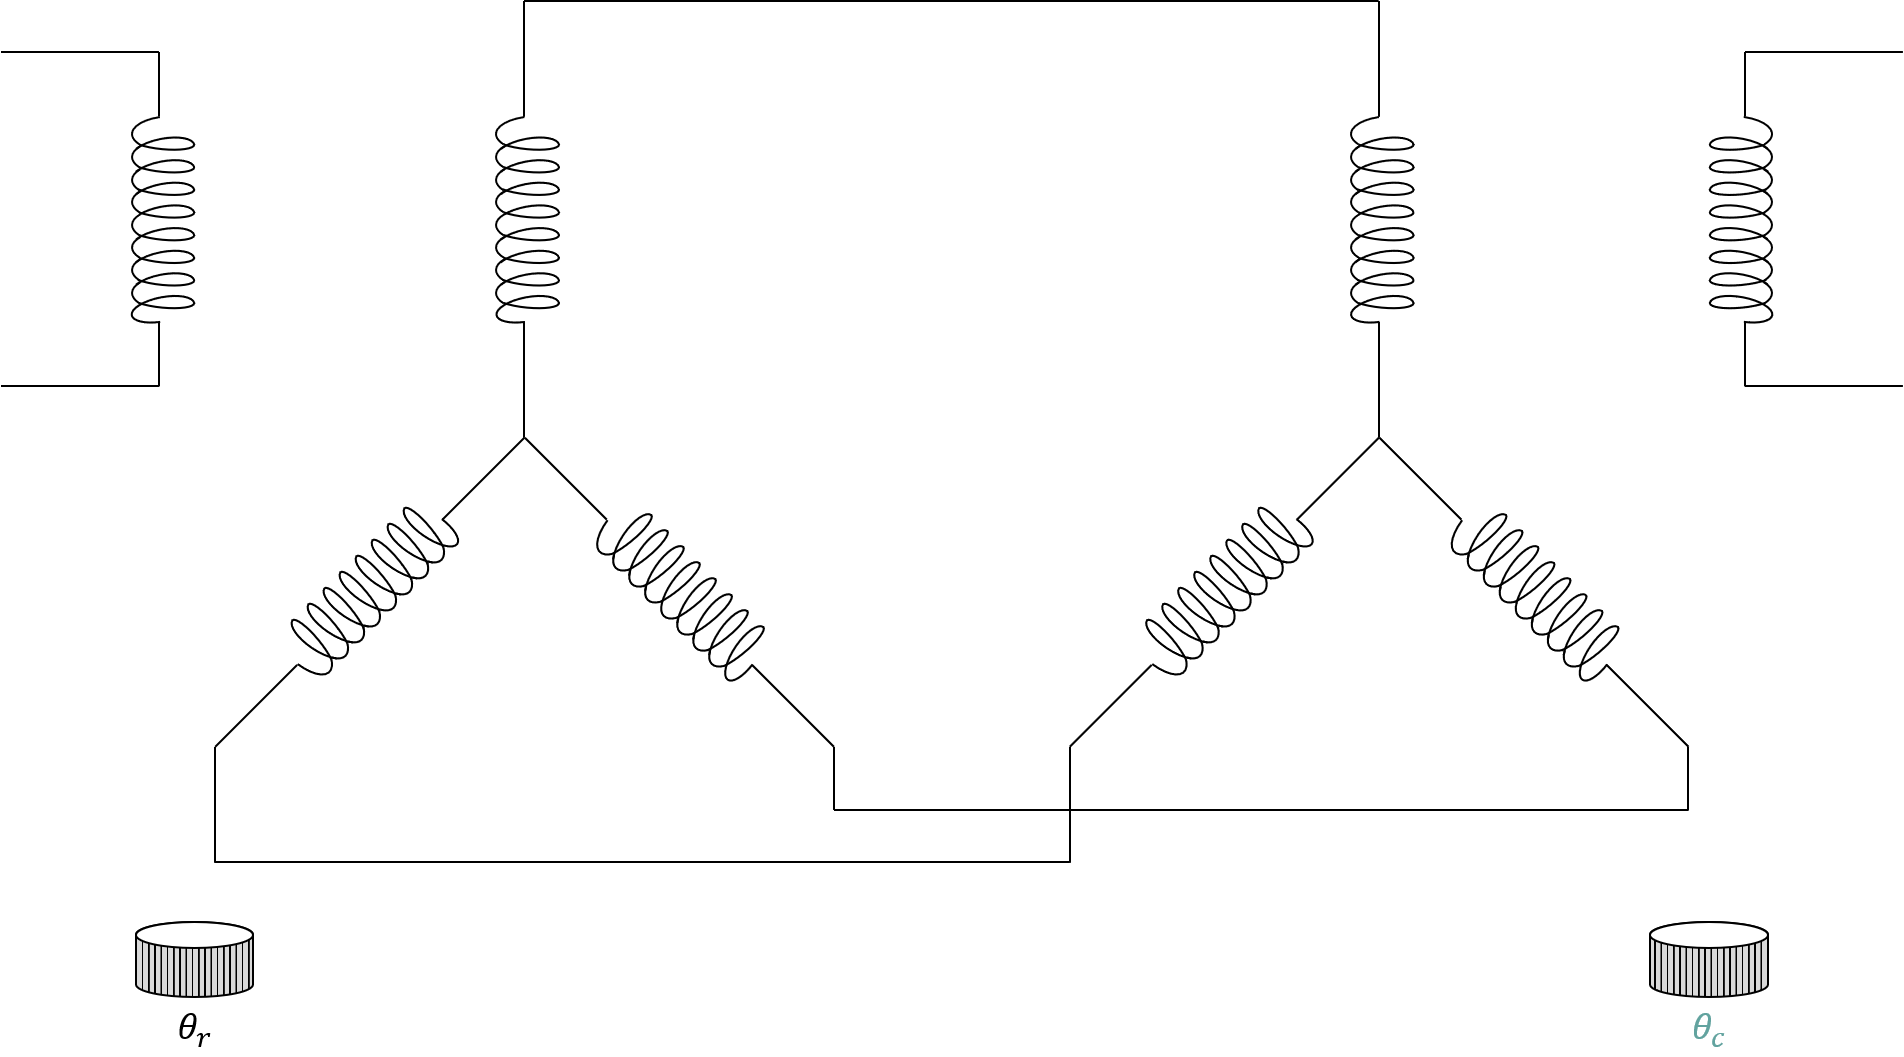
\includegraphics[height = 6.342 cm]{appendix_notSimpleSystemsEquations/Synchro} \\
		        \multicolumn{2}{c}{}\\[-1em]
		        \hline
		    \end{tabular}
\end{table}
				

\begin{description}
\item[Reference] Modern control systems.\footnote{Tables 2-4 ``International Edition''}
			\\\note{Richard c. Dorf, Robert h.Bishop}
\end{description}

\pagebreak